\graphicspath{{images/}}

\section*{Entscheidbarkeit}

\begin{definition}{Entscheidbar} $\exists$ Algorithmus, der $\forall$ Eingabe eine Antwort liefert
        
        \emph{Semi-entscheidbar}: $\exists$ Algorithmus, der $\forall$ Eingabe eine Antwort liefert, falls Antwort die Antwort «Ja» ist
    
\end{definition}

\begin{theorem}{Entscheidbarkeit} einer Sprache $A \subset \Sigma^{*}$

    $A \subset \Sigma^{*}$ ist entscheidbar $\Leftrightarrow$ $A$ und $\bar{A}$ sind semi-entscheidbar

    \vspace{1mm}

    {\small $\bar{A}=\Sigma^{*} \backslash A=\{\omega \in \Sigma^{*} \mid \omega \notin A\}$ (Komplement von $A$)}

\end{theorem}

\begin{concept}{Entscheidbarkeit mit Turingmaschinen}

    $A \subset \Sigma^{*}$ heisst entscheidbar, wenn TM $T$ existiert, sodass:
    \begin{itemize}
    \item Bandinhalt $x \in A \quad T$ hält mit Bandinhalt «1» (Ja) an
    \item Bandinhalt $x \in \Sigma^{*} \backslash A \quad T$ hält mit Bandinhalt «0» (Nein) an
    \end{itemize}

    \vspace{1mm}

    {\small
    Äquivalente Aussagen: $A \subset \Sigma^{*}$ ist entscheidbar
    \begin{itemize}
        \item Es existiert eine $T M$, die das Entscheidungsproblem $T(\Sigma, A)$ löst
        \item Es existiert ein WHILE-Programm, dass bei einem zu $A$ gehörenden Wort stets terminiert $\rightarrow$ Entscheidungsverfahren für $A$
    \end{itemize}
    }
\end{concept}

\begin{concept}{Semi-Entscheidbarkeit mit Turingmaschinen}\\
    $A \subset \Sigma^{*}$ heisst semi-entscheidbar, wenn TM $T$ existiert, sodass:

    \begin{itemize}
    \item Bandinhalt $x \in A \quad T$ hält mit Bandinhalt «1» (Ja) an
    \item Bandinhalt $x \in \Sigma^{*} \backslash A \quad T$ hält nie an
    \end{itemize}

    \vspace{1mm}

    {\small
    Äquivalente Aussagen: $A \subset \Sigma^{*}$ ist semi-entscheidbar
    \begin{itemize}
    \item $A \subset \Sigma^{*}$ ist rekursiv aufzählbar
    \item Es gibt eine TM, die zum Entscheidungsproblem $T(\Sigma, A)$ nur die positiven («Ja») Antworten liefert und sonst gar keine Antwort
    \item Es gibt ein WHILE-Programm, dass bei einem zu $A$ gehörenden Wort stets terminiert und bei Eingabe von Wörtern die nicht zu $A$ gehören nicht terminiert
    \end{itemize}
    }
\end{concept}

\begin{theorem}{Reduktion} $A \preccurlyeq B \quad \Rightarrow A \subset \Sigma^{*}$ reduzierbar auf $B \subset \Gamma^{*}$

    Gilt wenn  $\exists$ $T: \Sigma^{*} \rightarrow \Gamma^{*}$ so dass: $\forall \omega \in \Sigma^{*} \quad \omega \in A \Leftrightarrow F(\omega) \in B$
    
    {\footnotesize T := total Turing-berechenbare Funktion}

    \vspace{1mm}

    Eigenschaften:
    
    Transitiv: $A \preccurlyeq B$ und $B \preccurlyeq C \rightarrow A \preccurlyeq C$

    $A \preccurlyeq B \Rightarrow$ Entscheidbarkeit von $B$ gleich wie von $A$
\end{theorem}

\begin{concept}{Halteproblem}
    Ist es möglich einen Algorithmus zu schreiben, der für jede TM entscheiden kann, ob sie hält oder nicht? (Nein!)
    
    \vspace*{1mm}

    Halteprobleme (HP) definiert als Sprachen: {\small(\# = Delimiter)}

    \vspace*{1mm}

    \emph{Allgemeines} $H :=\{\omega \# x \in\{0,1, \#\}^{*} \mid T_{\omega} \text{ angesetzt auf } x \text{ hält} \}$

    \emph{Leeres} $H_{0}:=\{\omega \in\{0,1\}^{*} \mid T_{\omega}$ angesetzt auf das leere Band hält $\}$ 
    
    \emph{Spezielles} $H_{S}:=\{\omega \in\{0,1\}^{*} \mid T_{\omega}$ angesetzt auf $\omega$ hält $\}$

    \vspace*{1mm}

    {\small
    $H_{0} \preccurlyeq H_{S} \preccurlyeq H$

    $H_{0}, H_{S}$ und $H$ sind semi-entscheidbar und nicht entscheidbar.
    }
\end{concept}

\begin{center}
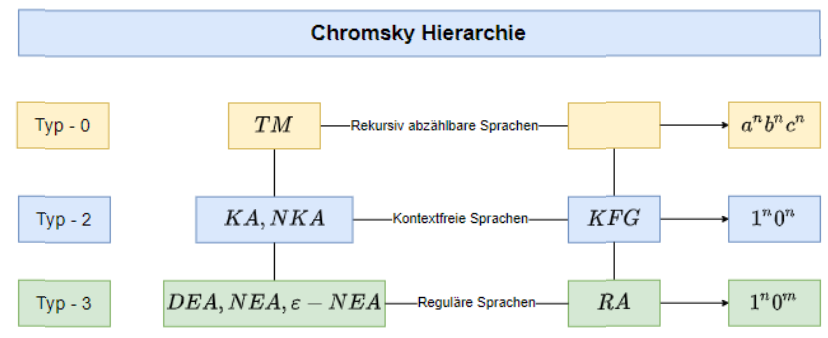
\includegraphics[width=1\linewidth]{chomsky_hierarchie.png}
\end{center}